% --- Slide 1: Hypothesis & Setup for Edge Case ---
\begin{frame}{Failure Mode Experiment: Dental Braces}
    \begin{columns}[T]
        \begin{column}{0.50\textwidth}
            \begin{block}{Experiment Setup}
                \small
                \begin{itemize}
                    \item \textbf{Test Idea:} How does FOMM handle rare facial features absent from training data?
                    \item \textbf{Subject:} Source portrait with metallic dental braces (\texttt{bella\_poarch\_dis\_teli}).
                    \item \textbf{Driving Motion:} Sequences from subtle head tilt to closed mouth, ending in a wide squinting smile.
                \end{itemize}
            \end{block}
        \end{column}

        \begin{column}{0.48\textwidth}
            \begin{block}{Hypothesis}
                \small
                \begin{itemize}
                    \item VoxCeleb training data has virtually zero faces with dental braces.
                    \item \textbf{Warping Regime ($O \approx 1$):} Optical flow copies real source pixels $\to$ braces preserved.
                    \item \textbf{Inpainting Regime ($O \approx 0$):} Under extreme deformation, model flags teeth as occluded and synthesizes them.
                    \item \textbf{Prediction:} Inpainting will sample dataset average and erase braces.
                \end{itemize}
            \end{block}
        \end{column}
    \end{columns}
\end{frame}

% --- Slide 2: Visual Evidence of Failure Mode (3x3 Grid) ---
\begin{frame}{Failure Mode: Vanishing Dental Braces}
    \begin{columns}[c]
        \begin{column}{0.54\textwidth}
            \centering
            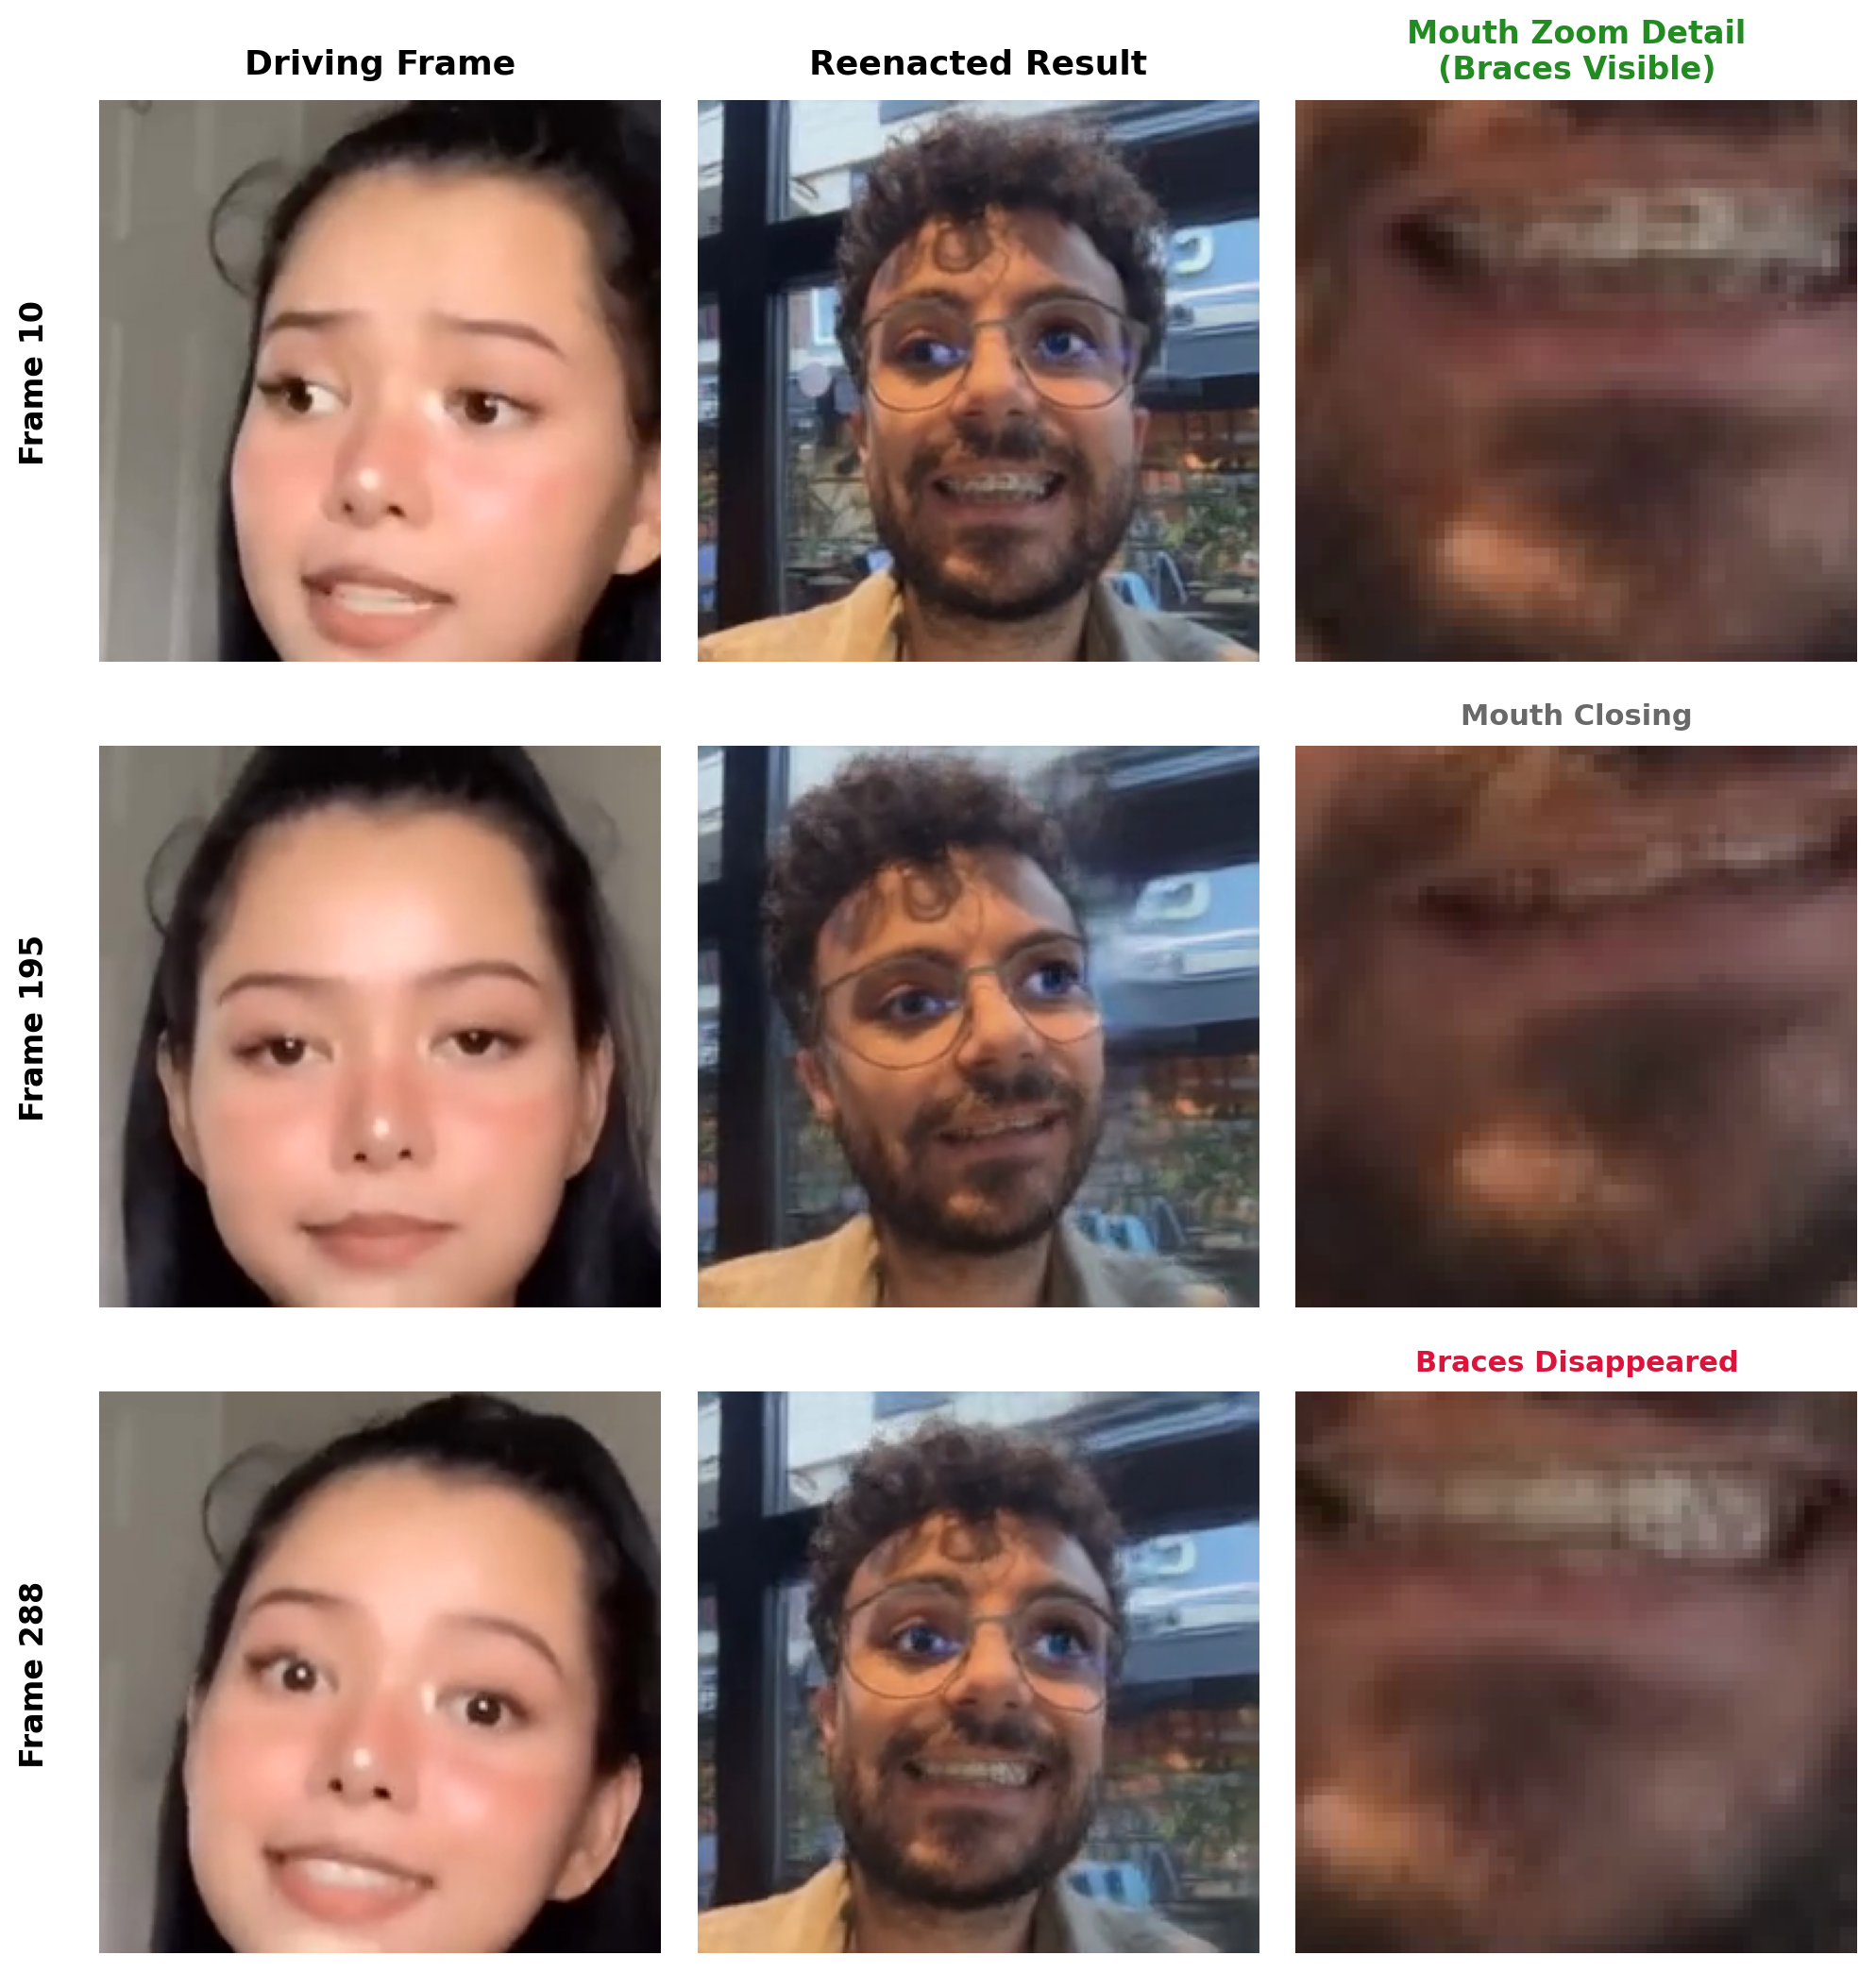
\includegraphics[width=\linewidth, height=5.2cm, keepaspectratio]{dis_teli_kaybolma_analizi.png}
            \vspace{0.05cm}
            
            \scriptsize \textit{Frame 10 (top), Frame 195 (middle), Frame 288 (bottom).}
        \end{column}

        \begin{column}{0.44\textwidth}
            \textbf{Observation Across Frames:}
            \begin{itemize}
                \item \textbf{Frame 10 (0.3s) — Warping:} Small motion offset; teeth mapped from source ($O \approx 1$). Metallic brackets intact.
                \item \textbf{Frame 195 (6.5s) — Natural Closure:} Driving mouth closes; teeth hidden behind lips.
                \item \textbf{Frame 288 (9.6s) — Inpainting Failure:} Wide squint/smile exceeds flow limits $\to$ mouth flagged as occluded ($O \approx 0$).
                \item Generator draws standard white teeth from dataset prior; \textbf{braces vanish completely}.
            \end{itemize}
        \end{column}
    \end{columns}
\end{frame}

% --- Slide 3: Root Cause Analysis & Video Links ---
\begin{frame}{Root Cause: Why Did It Fail?}
    \begin{columns}[T]
        \begin{column}{0.50\textwidth}
            \begin{block}{Technical Causes}
                \small
                \begin{enumerate}
                    \item \textbf{Stateless Generation:} Each frame is computed strictly from $(S, D_t)$. Frame 195 does not cause Frame 288's loss; Frame 288 fails due to its own extreme deformation mismatch.
                    \item \textbf{Dataset Bias in Inpainting:} When $O \approx 0$, generator ignores source pixels and samples from VoxCeleb average (normal teeth).
                    \item \textbf{Zero Identity Cache:} FOMM lacks recurrent memory to inject known identity traits into the inpainter.
                \end{enumerate}
            \end{block}
        \end{column}

        \begin{column}{0.46\textwidth}
            \begin{block}{Main Takeaway}
                \small
                \begin{itemize}
                    \item \textbf{Warping} preserves unique personal traits.
                    \item \textbf{Inpainting} pulls outputs toward dataset averages.
                    \item \textbf{Architectural Fix:} Requires 3D geometry priors or persistent identity memory.
                \end{itemize}
            \end{block}

            \vspace{0.15cm}
            \begin{block}{Braces Experiment Videos}
                \small
                \begin{itemize}
                    \item \textbf{Side-by-Side Video:} \href{https://YOUR-EXTERNAL-VIDEO-LINK-HERE}{\underline{\textcolor{primaryNavy}{Watch Online (External Link)}}}
                    \item \textbf{Reenacted Result:} \href{https://YOUR-EXTERNAL-VIDEO-LINK-HERE}{\underline{\textcolor{primaryNavy}{Watch Online (External Link)}}}
                \end{itemize}
            \end{block}
        \end{column}
    \end{columns}
\end{frame}
